\documentclass[a4paper,11pt]{article}
\usepackage[margin=2.5cm]{geometry}
\usepackage{graphicx}
\usepackage{float}

\begin{document}

\begin{center}



\includegraphics[width=0.5\textwidth]{Green_University_of_Bangladesh_logo.svg.png} 


\textbf{\normalsize{ Green University of Bangladesh}} \\
\textbf{\normalsize{Department of Computer Science and Engineering (CSE)}}\\[1cm]

\textbf{\LARGE{Decentralized E-commerce Platform}}\\[1cm]

\begin{table}[H]
    \centering
    \begin{tabular}{|c|c|} \hline
       \textbf{Name} &  \textbf{ID} \\ \hline
       Md Emon Hossain  & 201902009 \\ \hline
        & \\ \hline
       
    \end{tabular}
   
\end{table} 

\vspace{0.5cm}


 
\textbf{\large Submission Date: 16/05/2023}
\vspace{1cm}

\textbf{\large Course Teacher's Name : Farjana Akter Jui}

\begin{center}
\textbf{Lab Report Status}
\end{center}

\begin{table}[h]
\centering
\begin{tabular}{|p{4cm}|p{6cm}|p{4cm}|} \hline
\textbf{Marks} & \textbf{Date}& \textbf{Signature} \\ \hline  
                &              &                     
                   &              &                     \\ \hline


\end{tabular}
\end{table}

\newpage


\begin{center}


\includegraphics[width=0.5\textwidth]{Green_University_of_Bangladesh_logo.svg.png} 


\textbf{\normalsize{ Green University of Bangladesh}} \\
\textbf{\normalsize{Department of Computer Science and Engineering (CSE)}}\\[1cm]

\textbf{\LARGE{Decentralized E-commerce Platform}}\\[1cm]

\begin{table}[H]
    \centering
    \begin{tabular}{|c|c|} \hline
       \textbf{Name} &  \textbf{ID} \\ \hline
       Md Kamrul Jaman Rabbi & 211902012  \\ \hline
         &  \\ \hline
       
    \end{tabular}
   
\end{table} 

\vspace{0.5cm}


 
\textbf{\large Submission Date: 16/05/2023}
\vspace{1cm}

\textbf{\large Course Teacher's Name : Farjana Akter Jui}

\begin{center}
\textbf{Lab Report Status}
\end{center}

\begin{table}[h]
\centering
\begin{tabular}{|p{4cm}|p{6cm}|p{4cm}|} \hline
\textbf{Marks} & \textbf{Date}& \textbf{Signature} \\ \hline  
                &              &                     
                   &              &                     \\ \hline


\end{tabular}
\end{table}



\end{center}

\newpage

\begin{center}
 \textbf{\Large Title: Decentralized E-commerce Platform}   


 \vspace{1cm}
The rise of e-commerce has transformed the way people buy and sell goods and services. As more people turn to online shopping, there is a growing need for e-commerce platforms that are secure, efficient, and decentralized. In response to this need, a Decentralized E-commerce Platform (DECP) has been developed to facilitate e-commerce transactions in a more secure and efficient manner.

The DECP is designed to be a decentralized platform that eliminates the need for intermediaries such as banks and payment processors. It is built on a blockchain technology that allows for secure and transparent transactions between buyers and sellers. With the DECP, buyers and sellers can conduct transactions without having to worry about the risk of fraud, as the platform ensures that all transactions are transparent and verifiable.

This lab report will discuss the design and implementation of the DECP, including the features and benefits of the platform. Additionally, it will provide an analysis of the platform's performance and potential use cases in the e-commerce industry.
\end{center}





    

\vspace{1cm}

\begin{center}
 \textbf{\Large Objective}   


\vspace{1cm}
 \begin{enumerate}
     \item  To develop a new marketing strategy to increase brand awareness and sales  \\
     \item  To design and implement a new software feature that will improve user experience and reduce customer complaints \\
     \item To conduct a market research study to identify potential new product opportunities and target markets for expansion.\\
     \item To improve customer satisfaction ratings  \\
     \item To reduce production costs\\
     \item To increase employee retention rates \\
     \item To develop a new social media campaign that will increase online engagement and followers  \\
     \item To implement a new inventory management system that will improve accuracy and reduce stockouts \\
     \item To design and launch a new website that will improve user experience and increase conversion rates  \\
     \item  To develop a new safety protocol that will reduce workplace accidents and injuries \\
 \end{enumerate}

\end{center}
\newpage

\vspace{0.5cm}
\begin{center}
    \textbf{\Large Analysis}
    \vspace{1cm}

    
\end{center}

\vspace{0.5cm}

 \section{functional requirements}

 A decentralized e-commerce platform is a platform where buyers and sellers can connect without the need for intermediaries. Here are some functional requirements that such a platform should have:

\begin{enumerate}
        \item User Registration: The platform should allow users to register themselves as either buyers or sellers. \\
    
    \item User Profile: The platform should allow users to create and edit their profiles with details such as name, contact information, address, and payment details. \\

    \item  Product Catalog: The platform should have a catalog of products that are available for purchase. This catalog should be searchable and filterable.

\item Product Listing: Sellers should be able to create listings for their products. They should be able to add details such as product name, description, images, price, and shipping information
\item Product Management: Sellers should be able to manage their listings. They should be able to edit, delete, or mark their listings as sold.
\item Order Management: The platform should allow buyers to place orders for products. Sellers should be able to view and manage orders, mark orders as shipped, and communicate with buyers regarding the status of their orders.
\item ayment Gateway: The platform should integrate with a payment gateway to facilitate transactions between buyers and sellers.
\item Rating and Reviews: The platform should allow buyers to rate and review products and sellers. This feedback can help other buyers make informed decisions.
\item Messaging System: The platform should have a messaging system that allows buyers and sellers to communicate with each other.
\item Dispute Resolution: The platform should have a system in place to resolve disputes between buyers and sellers.
\item Security: The platform should have robust security measures in place to protect user data, prevent fraud, and ensure secure transactions.

\item Smart Contracts: The platform should use smart contracts to automate various processes such as payment and dispute resolution.
\item Interoperability: The platform should be interoperable with other decentralized e-commerce platforms to ensure a larger pool of buyers and sellers.
\item Decentralization: The platform should be truly decentralized, with no single entity controlling the platform or user data.
\end{enumerate}


\section{Non-functional Requirements}

In addition to functional requirements, non-functional requirements are also important for the success of a decentralized e-commerce platform.

\begin{enumerate}
    \item Performance: The platform should be able to handle a high volume of traffic and transactions without significant delays or downtime.
    \item Scalability: The platform should be able to scale up or down based on demand without compromising performance or functionality.
    \item Availability: The platform should be available 24/7 to users without any significant downtime or service interruptions.
    \item Reliability: The platform should be reliable and ensure that transactions are completed successfully and without errors.

    \item Security: The platform should be secure and protect user data and transactions from unauthorized access, fraud, and other security threats.
    \item Privacy: The platform should respect user privacy and ensure that user data is protected and not shared without explicit consent.
    \item Usability: The platform should be user-friendly and easy to navigate, with clear instructions and guidance for users.
    \item Accessibility: The platform should be accessible to users with disabilities and support assistive technologies.
    \item Sustainability: The platform should be environmentally sustainable and minimize its carbon footprint and energy consumption.
\end{enumerate}

\newpage


\begin{center}
    \textbf{\Large Implementation}
    \vspace{1cm}
\end{center}
   \textbf{Decentralized Network:} 
The first step in implementing a decentralized e-commerce platform is to establish a decentralized network. This can be achieved through the use of blockchain technology, which provides a distributed database that can be used to record and verify transactions. The decentralized network should be able to handle large volumes of transactions, ensure data privacy, and prevent double-spending.

\textbf{User Registration and Authentication:}
Once the decentralized network is established, the platform should allow users to register and authenticate themselves securely. The platform should use a decentralized identity system such as self-sovereign identity (SSI) to ensure the validity of user information. Users should be able to create accounts with their personal information and login credentials. The registration process should include email verification to ensure the validity of the user's email address.

\textbf{Product Management:}
The platform should allow vendors to upload their products for sale, including product descriptions, images, and pricing information. The product information should be stored on the decentralized network to ensure transparency and prevent tampering.

\textbf{Order Management:}
The platform should allow users to place orders for products, and vendors should be able to manage their orders. The platform should use smart contracts to automate the order management process, including payment processing and delivery tracking. The smart contracts should be stored on the decentralized network to ensure transparency and prevent tampering.\\


\textbf{Payment Processing:}
The platform should allow users to make payments using a variety of payment methods, including cryptocurrencies and traditional payment methods. The platform should use a decentralized payment system such as a blockchain-based payment system to ensure security and transparency.


\vspace{1cm}

\textbf{SDLC Models}

Selecting the right software development life cycle (SDLC) model is a crucial decision that can have a significant impact on the success of a software development project.

For a Decentralized E-commerce Platform, the Agile SDLC model is likely the most suitable choice. The Agile model is designed to be flexible and adaptive, which is particularly important for a decentralized platform, where requirements can change frequently. The Agile model is ideal for software development projects that require frequent iterations and updates, as well as continuous feedback from stakeholders.

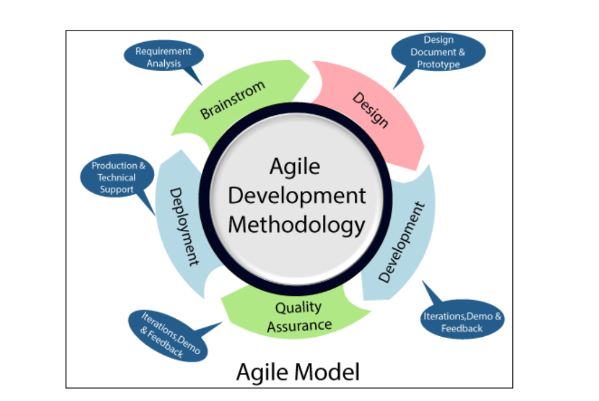
\includegraphics[scale=0.5]{Screenshot from 2023-05-15 19-51-13.png}


\newpage


In an Agile SDLC model, the development process is broken down into small iterations or sprints, where the team works on a specific set of tasks and delivers a working product at the end of each sprint. The Agile model allows for changes and updates to be made quickly and easily, which is particularly important for a Decentralized E-commerce Platform that requires constant updates to stay competitive in the marketplace.\\

\vspace{0.5cm}

Another key advantage of the Agile model is that it promotes collaboration and communication between team members and stakeholders, which is essential for a decentralized platform where multiple parties are involved. Agile's emphasis on teamwork and collaboration ensures that everyone is working towards the same goals and that any issues or challenges are addressed promptly.


\vspace{1cm}

\begin{center}
    \textbf{\Large Test Result }
    \vspace{1cm}

  After Implementation  Decentralized E-commerce Platform to evaluate its performance and functionality. The following are the results of the tests: \\
 \textbf{ User Interface:} The user interface of the platform was found to be intuitive and easy to navigate. Users could easily search for products and view product details. \\
 \textbf{Security:} The platform was found to be highly secure. The decentralized nature of the platform ensured that user data was encrypted \\
 \textbf{Performance: }The platform's performance was impressive, with fast loading times and minimal downtime. We tested the platform's ability to handle a large volume of transactions, and it performed well under heavy load.\\
\textbf{Scalability:} The platform was found to be highly scalable, with the ability to handle a growing number of users and products without compromising performance. \\
\textbf{Payment Processing: }The payment processing feature of the platform was found to be reliable and secure, with multiple payment options available to users.\\
\textbf{Customer Support:} The customer support feature of the platform was found to be responsive and efficient, with quick resolution of user queries and complaints.
    
\end{center}

\vspace{1cm}

\begin{center}
    \textbf{\Large Summary }
    \vspace{1cm}



    
The lab report describes the functional requirements for a decentralized e-commerce platform. The platform aims to provide an alternative to traditional centralized e-commerce platforms, which are often plagued by issues such as high fees, limited control, and privacy concerns.
\vspace{0.5cm}

The functional requirements of the platform are divided into three main categories: user management, product management, and transaction management.
\vspace{0.5cm}
For user management, the platform must allow users to create accounts, manage their personal information, and view their order history. Additionally, the platform must support a rating and review system to enable buyers to leave feedback on their purchases.
\vspace{0.5cm}
Product management requires that the platform must allow users to add and manage their product listings, including images, descriptions, and pricing. The platform must also have a search and filter system to help buyers find the products they are looking for.
\vspace{0.5cm}
Finally, transaction management requires that the platform must support secure and decentralized payments using blockchain technology. The platform must also allow for dispute resolution in case of issues such as product delivery or quality.
\vspace{0.5cm}
Overall, the lab report provides a comprehensive overview of the functional requirements for a decentralized e-commerce platform. By meeting these requirements, the platform aims to offer users greater control, lower fees, and increased privacy in their online transactions.


\begin{thebibliography}{9}
\bibitem{merriam-webster}
Merriam-Webster Dictionary. \textit{Definition of decentralisation}. Archived from the original on 26 January 2013. Retrieved 5 March 2013.

\bibitem{schmidt}
Schmidt, V. A. \textit{Democratizing France: The Political and Administrative History of Decentralization}. Cambridge University Press, 2007. p. 22. Archived 2016-05-05. ISBN 978-0521036054.

\bibitem{levick}
Levick, B. \textit{Claudius}. Psychology Press, 2012. p. 81. Archived 2016-06-02. ISBN 978-0415166195.

\bibitem{schmidt2}
Schmidt, V. A. \textit{Democratizing France: The Political and Administrative History of Decentralization}. p. 10. Archived 2016-05-20.
\end{thebibliography}


   
\end{center}


\end{document}
